\documentclass{beamer}
\usetheme{metropolis}           % Use metropolis theme
\metroset{numbering=fraction}
\usepackage{tikz}
\usetikzlibrary{arrows,positioning,shapes.geometric}
\usepackage{float}
\usepackage{makecell}
\usepackage{fancyvrb}
\usepackage{listings}
\usepackage[export]{adjustbox}
\usepackage{caption}
\title{Lecture 2 \\ Introduction to Object-Oriented Programming (OOP) and Java}
\date{\today}
\author{Patrick Lam \\ Jeff Zarnett \\ Michael Giannikouris}
\institute{Department of Electrical and Computer Engineering}
\setbeamertemplate{caption}{\raggedright\insertcaption\par}
\setbeamersize{text margin left=12pt,text margin right=12pt}
\newcommand{\putat}[3]{\begin{picture}(0,0)(0,0)\put(#1,#2){#3}\end{picture}} % just a shorthand

\newenvironment{deflist}
{ \begin{description}
    \setlength{\itemsep}{6pt}
    \setlength{\parskip}{0pt}
    \setlength{\parsep}{0pt}     }
{ \end{description}                  } 

\newenvironment{splitslide}
{
\centering
\begin{tabular}{@{}p{0.50\textwidth} | p{0.025\textwidth}@{} p{0.4\textwidth}@{}}
}
{
\end{tabular}
}


\begin{document}
\maketitle

\section{Characteristics of OOP}

%%%%%%%%%%%%%%%%%%%%%%%%%%%%%%%%%%%%%%%%%%%%%%%%%%%%%%%%%%%%%%%%%%%%%%%%%%%%%%%%%%%%
% Encapsulation (Definition)
%%%%%%%%%%%%%%%%%%%%%%%%%%%%%%%%%%%%%%%%%%%%%%%%%%%%%%%%%%%%%%%%%%%%%%%%%%%%%%%%%%%%
\begin{frame}{Characteristics of OOP}
	\begin{deflist}
		\item[Encapsulation]
		Data and methods that operate on the data are \textbf{bundled} together in a single container.	
		\item Some of the data and methods internal to the container may be hidden, depending on their \textbf{visibility}.
		\item[] Typically, OOP languages (including Java) call this container a \textbf{class}.
	\end{deflist}
\end{frame}
%%%%%%%%%%%%%%%%%%%%%%%%%%%%%%%%%%%%%%%%%%%%%%%%%%%%%%%%%%%%%%%%%%%%%%%%%%%%%%%%%%%%



%%%%%%%%%%%%%%%%%%%%%%%%%%%%%%%%%%%%%%%%%%%%%%%%%%%%%%%%%%%%%%%%%%%%%%%%%%%%%%%%%%%%
% Encapsulation (Bundling)
%%%%%%%%%%%%%%%%%%%%%%%%%%%%%%%%%%%%%%%%%%%%%%%%%%%%%%%%%%%%%%%%%%%%%%%%%%%%%%%%%%%%
\begin{frame}[fragile]{Encapsulation}

\centering
\begin{tabular}{@{}m{0.50\textwidth} | m{0.03\textwidth}@{} m{0.4\textwidth}@{}}

\begin{Verbatim}[fontsize=\tiny]
public class BankAccount {
  public double balance;
  
  // deposit an amount
  public void deposit(double amount) {
    balance += amount;
  }
  
  // withdraw an amount
  public boolean withdraw(double amount) {
    if(balance < amount) {
      return false;
    }
    else {
      balance -= amount;
      return true;
    }
  }
}
\end{Verbatim}

&&

\raggedright
\begin{footnotesize}
Data (\textbf{balance}) 	\\
and methods (\textbf{deposit}, \textbf{withdraw})	\\
are \textbf{bundled} into a single container, the BankAccount \textbf{class}. \\
\end{footnotesize}

\end{tabular}

\end{frame}
%%%%%%%%%%%%%%%%%%%%%%%%%%%%%%%%%%%%%%%%%%%%%%%%%%%%%%%%%%%%%%%%%%%%%%%%%%%%%%



%%%%%%%%%%%%%%%%%%%%%%%%%%%%%%%%%%%%%%%%%%%%%%%%%%%%%%%%%%%%%%%%%%%%%%%%%%%%%%
% Encapsulation (Visibility)
%%%%%%%%%%%%%%%%%%%%%%%%%%%%%%%%%%%%%%%%%%%%%%%%%%%%%%%%%%%%%%%%%%%%%%%%%%%%%%
\begin{frame}[fragile]{Encapsulation}

\centering
\begin{tabular}{@{}m{0.50\textwidth} | m{0.03\textwidth}@{} m{0.4\textwidth}@{}}

\begin{Verbatim}[fontsize=\tiny]
public class BankAccount {
  public double balance;
  
  // deposit an amount
  public void deposit(double amount) {
    balance += amount;
  }
  
  // withdraw an amount
  public boolean withdraw(double amount) {
    if(balance < amount) {
      return false;
    }
    else {
      balance -= amount;
      return true;
    }
  }
}
\end{Verbatim}

&&

\raggedright
\begin{footnotesize}
Notice that we've put \textbf{public} in front of all of our data and methods (and the class itself). \\
\vspace{0.5em}
Public is one of Java's \textbf{access modifier} keywords. \\
\vspace{0.5em}
These keywords control the \textbf{visibility} of class members (and classes themselves). 
\end{footnotesize}

\end{tabular}

\end{frame}
%%%%%%%%%%%%%%%%%%%%%%%%%%%%%%%%%%%%%%%%%%%%%%%%%%%%%%%%%%%%%%%%%%%%%%%%%%%%%%%%%%%%



%%%%%%%%%%%%%%%%%%%%%%%%%%%%%%%%%%%%%%%%%%%%%%%%%%%%%%%%%%%%%%%%%%%%%%%%%%%%%%%%%%%%
% Java Access Modifiers 
%%%%%%%%%%%%%%%%%%%%%%%%%%%%%%%%%%%%%%%%%%%%%%%%%%%%%%%%%%%%%%%%%%%%%%%%%%%%%%%%%%%%
\begin{frame}[fragile]{Java Access Modifiers}
\begin{center}
\begin{tabular}{ l | l | l | l | l }
\textbf{Modifier} & \textbf{Class} & \textbf{Package} & \textbf{Subclass} & \textbf{World} \\
\hline
public & Y & Y & Y & Y \\
\hline
protected & Y & Y & Y & N \\
\hline
\textit{no modifier} & Y & Y & N & N \\
\hline
private & Y & N & N & N \\
\end{tabular}
\end{center}
\end{frame}
%%%%%%%%%%%%%%%%%%%%%%%%%%%%%%%%%%%%%%%%%%%%%%%%%%%%%%%%%%%%%%%%%%%%%%%%%%%%%%%%%%%%



%%%%%%%%%%%%%%%%%%%%%%%%%%%%%%%%%%%%%%%%%%%%%%%%%%%%%%%%%%%%%%%%%%%%%%%%%%%%%%
% Encapsulation (Choosing Good Visibility)
%%%%%%%%%%%%%%%%%%%%%%%%%%%%%%%%%%%%%%%%%%%%%%%%%%%%%%%%%%%%%%%%%%%%%%%%%%%%%%
\begin{frame}[fragile]{Encapsulation}

\centering
\begin{tabular}{@{}m{0.50\textwidth} | m{0.03\textwidth}@{} m{0.4\textwidth}@{}}

\begin{Verbatim}[fontsize=\tiny]
public class BankAccount {
  private double balance;
  
  // deposit an amount
  public void deposit(double amount) {
    balance += amount;
  }
  
  // withdraw an amount
  public boolean withdraw(double amount) {
    if(balance < amount) {
      return false;
    }
    else {
      balance -= amount;
      return true;
    }
  }
  
  // view balance
  public double view_balance() {
    return balance;  
  }
}
\end{Verbatim}

&&

\raggedright
\begin{footnotesize}
Visibility is very important when designing a class.\\
\vspace{0.5em}
For example, we probably don't want users to be able to directly change \textbf{balance}, so we'll make it \textbf{private}. \\
\vspace{0.5em}
If we're going to hide \textbf{balance}, we should make a public function to view the balance. In this way, we've made balance \textbf{read-only}. \\
\vspace{0.5em}
In general, use the most restrictive access level possible. \\
\end{footnotesize}

\end{tabular}

\end{frame}
%%%%%%%%%%%%%%%%%%%%%%%%%%%%%%%%%%%%%%%%%%%%%%%%%%%%%%%%%%%%%%%%%%%%%%%%%%%%%%%%%%%%



%%%%%%%%%%%%%%%%%%%%%%%%%%%%%%%%%%%%%%%%%%%%%%%%%%%%%%%%%%%%%%%%%%%%%%%%%%%%%%%%%%%%
% Inheritence 
%%%%%%%%%%%%%%%%%%%%%%%%%%%%%%%%%%%%%%%%%%%%%%%%%%%%%%%%%%%%%%%%%%%%%%%%%%%%%%%%%%%%
\begin{frame}{Characteristics of OOP}
	\begin{deflist}
		\item[Inheritance]
		Classes can \textbf{extend} (build on) other classes.
		\item[] A "child" class inherits (some of) the data and methods of the "parent" class.	
		\item[] A "child" class can also add new data and methods.
		\item[] In Java, we usually use the terms \textbf{superclass} and \textbf{subclass}.
	\end{deflist}
\end{frame}
%%%%%%%%%%%%%%%%%%%%%%%%%%%%%%%%%%%%%%%%%%%%%%%%%%%%%%%%%%%%%%%%%%%%%%%%%%%%%%%%%%%



%%%%%%%%%%%%%%%%%%%%%%%%%%%%%%%%%%%%%%%%%%%%%%%%%%%%%%%%%%%%%%%%%%%%%%%%%%%%%%%%%%%%
% Inheritence (subclassing)
%%%%%%%%%%%%%%%%%%%%%%%%%%%%%%%%%%%%%%%%%%%%%%%%%%%%%%%%%%%%%%%%%%%%%%%%%%%%%%%%%%%%
\begin{frame}[fragile]{Inheritance}
\begin{splitslide}

\begin{Verbatim}[fontsize=\tiny]
public class BankAccount {
  protected double balance;
  
  // deposit an amount
  public void deposit(double amount) {
    balance += amount;
  }
  
  // withdraw an amount
  public boolean withdraw(double amount) {
    if(balance < amount) {
      return false;
    }
    else {
      balance -= amount;
      return true;
    }
  }
  
  // view balance
  public double view_balance() {
    return balance;  
  }
}
\end{Verbatim}

&&

\begin{Verbatim}[fontsize=\tiny]
class SavingsAccount extends BankAccount {
  private double interest_rate = 0.008;
  
  // apply the interest rate
  public void apply_interest() {
    balance *= interest_rate;
  }
}
\end{Verbatim}


\vspace{1.5em}
\raggedright
Anyone notice a slight change in \textbf{BankAccount}?

\end{splitslide}
\end{frame}
%%%%%%%%%%%%%%%%%%%%%%%%%%%%%%%%%%%%%%%%%%%%%%%%%%%%%%%%%%%%%%%%%%%%%%%%%%%%%%%%%%%



%%%%%%%%%%%%%%%%%%%%%%%%%%%%%%%%%%%%%%%%%%%%%%%%%%%%%%%%%%%%%%%%%%%%%%%%%%%%%%%%%%%
% Inheritance (more info)
%%%%%%%%%%%%%%%%%%%%%%%%%%%%%%%%%%%%%%%%%%%%%%%%%%%%%%%%%%%%%%%%%%%%%%%%%%%%%%%%%%%
\begin{frame}[fragile]{Inheritance}
\begin{splitslide}

\centering
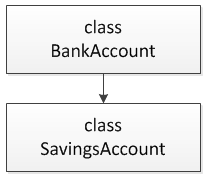
\includegraphics[scale=0.5]{img/single_inheritance.png}   \\
\vspace{2em}
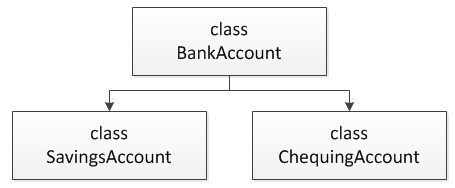
\includegraphics[scale=0.5]{img/single_inheritance_2.png}   \\

&&

\raggedright
\begin{footnotesize}
Java uses \textbf{single inheritance}, which means a subclass can extend a single superclass. \\
\vspace{1em}
In single inheritance, any number of subclasses can have the same superclass. \\
\end{footnotesize}

\end{splitslide}
\end{frame}
%%%%%%%%%%%%%%%%%%%%%%%%%%%%%%%%%%%%%%%%%%%%%%%%%%%%%%%%%%%%%%%%%%%%%%%%%%%%%%%%%%%



%%%%%%%%%%%%%%%%%%%%%%%%%%%%%%%%%%%%%%%%%%%%%%%%%%%%%%%%%%%%%%%%%%%%%%%%%%%%%%%%%%%
% Inheritance (more info)
%%%%%%%%%%%%%%%%%%%%%%%%%%%%%%%%%%%%%%%%%%%%%%%%%%%%%%%%%%%%%%%%%%%%%%%%%%%%%%%%%%%
\begin{frame}[fragile]{Inheritance}
\begin{splitslide}

\centering
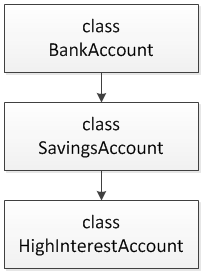
\includegraphics[scale=0.5]{img/multilevel_inheritance.png}   \\

&&

\raggedright
\begin{footnotesize}
Java also has \textbf{multi-level inheritance}, which means subclasses can themselves be subclassed. \\
\end{footnotesize}

\end{splitslide}
\end{frame}
%%%%%%%%%%%%%%%%%%%%%%%%%%%%%%%%%%%%%%%%%%%%%%%%%%%%%%%%%%%%%%%%%%%%%%%%%%%%%%%%%%%



%%%%%%%%%%%%%%%%%%%%%%%%%%%%%%%%%%%%%%%%%%%%%%%%%%%%%%%%%%%%%%%%%%%%%%%%%%%%%%%%%%%
% Inheritance (more info)
%%%%%%%%%%%%%%%%%%%%%%%%%%%%%%%%%%%%%%%%%%%%%%%%%%%%%%%%%%%%%%%%%%%%%%%%%%%%%%%%%%%
\begin{frame}[fragile]{Inheritance}
\begin{splitslide}

\centering
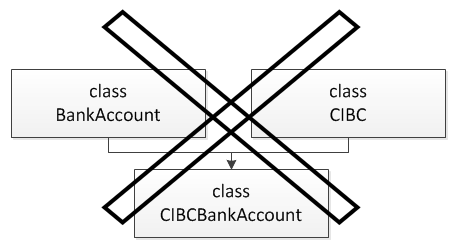
\includegraphics[scale=0.5]{img/multiple_inheritance.png}   \\

&&

\raggedright
\begin{footnotesize}
Java does \textbf{not} allow \textbf{multiple inheritance}...a class cannot inherit from multiple classes. \\
\vspace{0.5em}
There are certainly times where we want classes to take on behaviours or characteristics from multiple sources...there are better ways to do this that we will see. \\
\end{footnotesize}

\end{splitslide}
\end{frame}
%%%%%%%%%%%%%%%%%%%%%%%%%%%%%%%%%%%%%%%%%%%%%%%%%%%%%%%%%%%%%%%%%%%%%%%%%%%%%%%%%%%



%%%%%%%%%%%%%%%%%%%%%%%%%%%%%%%%%%%%%%%%%%%%%%%%%%%%%%%%%%%%%%%%%%%%%%%%%%%%%%%%%%%
% Polymorphism (definition)
%%%%%%%%%%%%%%%%%%%%%%%%%%%%%%%%%%%%%%%%%%%%%%%%%%%%%%%%%%%%%%%%%%%%%%%%%%%%%%%%%%%
\begin{frame}{Characteristics of OOP}
	\begin{description}
		\item[Polymorphism]
		A subclass can override (replace) a method inherited from the superclass with its own version.
	\end{description}
\end{frame}
%%%%%%%%%%%%%%%%%%%%%%%%%%%%%%%%%%%%%%%%%%%%%%%%%%%%%%%%%%%%%%%%%%%%%%%%%%%%%%%%%%%

%%%%%%%%%%%%%%%%%%%%%%%%%%%%%%%%%%%%%%%%%%%%%%%%%%%%%%%%%%%%%%%%%%%%%%%%%%%%%%%%%%%%
% Polymorphism (overriding)
%%%%%%%%%%%%%%%%%%%%%%%%%%%%%%%%%%%%%%%%%%%%%%%%%%%%%%%%%%%%%%%%%%%%%%%%%%%%%%%%%%%%
\begin{frame}[fragile]{Polymorphism}
\begin{splitslide}

\begin{Verbatim}[fontsize=\tiny]
public class BankAccount {
  protected double balance;
  
  // deposit an amount
  public void deposit(double amount) {
    balance += amount;
  }
  
  // withdraw an amount
  public boolean withdraw(double amount) {
    if(balance < amount) {
      return false;
    }
    else {
      balance -= amount;
      return true;
    }
  }
  
  // view balance
  public double view_balance() {
    return balance;  
  }
}
\end{Verbatim}

&&

\begin{Verbatim}[fontsize=\tiny]
class SavingsAccount extends BankAccount {
  private double interest_rate = 0.008;
  
  // apply the interest rate
  public void apply_interest() {
    balance *= interest_rate;
  }
}

class HighInterestAcct extends BankAccount {
  private double withdrawl_fee = 1.50;
  
  // override withdraw to add a fee
  public boolean withdraw(double amount) {
    int debit = amount + withdrawl_fee;    
    if(balance < debit) {
      return false;
    }
    else {
      balance -= debit;
      return true;
    }
  }
}
\end{Verbatim}

\end{splitslide}
\end{frame}
%%%%%%%%%%%%%%%%%%%%%%%%%%%%%%%%%%%%%%%%%%%%%%%%%%%%%%%%%%%%%%%%%%%%%%%%%%%%%%%%%%%%


\section{Working with Java Classes}


%%%%%%%%%%%%%%%%%%%%%%%%%%%%%%%%%%%%%%%%%%%%%%%%%%%%%%%%%%%%%%%%%%%%%%%%%%%%%%%%%%%%
% Objects
%%%%%%%%%%%%%%%%%%%%%%%%%%%%%%%%%%%%%%%%%%%%%%%%%%%%%%%%%%%%%%%%%%%%%%%%%%%%%%%%%%%%
\begin{frame}[fragile]{Objects}
Classes aren't any good unless we can use them. \\
\vspace{0.5em}
An object is an \textbf{instance} of a class.   \\
\vspace{0.5em}
Like variables, we can make as many instances of as many classes as memory allows. \\
	
\end{frame}
%%%%%%%%%%%%%%%%%%%%%%%%%%%%%%%%%%%%%%%%%%%%%%%%%%%%%%%%%%%%%%%%%%%%%%%%%%%%%%%%%%%%



%%%%%%%%%%%%%%%%%%%%%%%%%%%%%%%%%%%%%%%%%%%%%%%%%%%%%%%%%%%%%%%%%%%%%%%%%%%%%%%%%%%%
% Creating Objects
%%%%%%%%%%%%%%%%%%%%%%%%%%%%%%%%%%%%%%%%%%%%%%%%%%%%%%%%%%%%%%%%%%%%%%%%%%%%%%%%%%%%
\begin{frame}[fragile]{Creating objects}
We create an object in Java using the \textbf{new} keyword. \\
\vspace{0.5em}
\begin{Verbatim}
BankAccount my_account = new BankAccount();
\end{Verbatim}
\end{frame}
%%%%%%%%%%%%%%%%%%%%%%%%%%%%%%%%%%%%%%%%%%%%%%%%%%%%%%%%%%%%%%%%%%%%%%%%%%%%%%%%%%%%



%%%%%%%%%%%%%%%%%%%%%%%%%%%%%%%%%%%%%%%%%%%%%%%%%%%%%%%%%%%%%%%%%%%%%%%%%%%%%%%%%%%%
% Memory Management
%%%%%%%%%%%%%%%%%%%%%%%%%%%%%%%%%%%%%%%%%%%%%%%%%%%%%%%%%%%%%%%%%%%%%%%%%%%%%%%%%%%%
\begin{frame}[fragile]{Memory Management}
When you create an object in Java using the \textbf{new} keyword, two awesome things happen: \\
\begin{itemize}
\item[1] Java \textbf{automatically allocates memory} for the object (no calls to malloc()).
\item[2] Java \textbf{calls} the class' \textbf{constructor} to initialize the state of the object. \\
\end{itemize}
\end{frame}
%%%%%%%%%%%%%%%%%%%%%%%%%%%%%%%%%%%%%%%%%%%%%%%%%%%%%%%%%%%%%%%%%%%%%%%%%%%%%%%%%%%%



%%%%%%%%%%%%%%%%%%%%%%%%%%%%%%%%%%%%%%%%%%%%%%%%%%%%%%%%%%%%%%%%%%%%%%%%%%%%%%%%%%%%
% Constructors
%%%%%%%%%%%%%%%%%%%%%%%%%%%%%%%%%%%%%%%%%%%%%%%%%%%%%%%%%%%%%%%%%%%%%%%%%%%%%%%%%%%%
\begin{frame}[fragile]{Constructors}
\begin{splitslide}

\centering
\begin{Verbatim}[fontsize=\tiny]
public class BankAccount {
  protected double balance;
  
  // constructor
  public BankAccount(double opening_balance) {
    balance = opening_balance;
  }  

  // deposit an amount
  public void deposit(double amount) {
    balance += amount;
  }
  
  // withdraw an amount
  public boolean withdraw(double amount) {
    if(balance < amount) {
      return false;
    }
    else {
      balance -= amount;
      return true;
    }
  }
  
  // view balance
  public double view_balance() {
    return balance;  
  }
}
\end{Verbatim}

&&

\raggedright
\begin{footnotesize}
In Java, a constructor is a method inside a class that has, simply, the name of the class (and no return type). \\
\vspace{0.5em}
A constructor may take none, one, or may arguments. \\
\vspace{0.5em}
A class can have multiple (overloaded) constructors. \\
\vspace{0.5em}
A subclass can override the constructor(s) of the superclass. \\
\vspace{0.5em}
If you do not write a constructor, Java will call a default constructor, initializing everything to zero, false, null, etc. \\
\end{footnotesize}

\end{splitslide}
\end{frame}
%%%%%%%%%%%%%%%%%%%%%%%%%%%%%%%%%%%%%%%%%%%%%%%%%%%%%%%%%%%%%%%%%%%%%%%%%%%%%%%%%%%%



%%%%%%%%%%%%%%%%%%%%%%%%%%%%%%%%%%%%%%%%%%%%%%%%%%%%%%%%%%%%%%%%%%%%%%%%%%%%%%%%%%%%
% Memory Management
%%%%%%%%%%%%%%%%%%%%%%%%%%%%%%%%%%%%%%%%%%%%%%%%%%%%%%%%%%%%%%%%%%%%%%%%%%%%%%%%%%%%
\begin{frame}[fragile]{Memory Management}
To further "free" you from managing memory, Java uses garbage collection to free up memory that is no longer used. \\
\vspace{0.5em}
Java keeps track of objects that are in use. When an object is no longer being referred to, its memory is automatically freed. \\
\vspace{0.5em}
The inner workings of garbage collection are beyond this course....just rest easy knowing you don't really have to worry about memory. \\
\end{frame}
%%%%%%%%%%%%%%%%%%%%%%%%%%%%%%%%%%%%%%%%%%%%%%%%%%%%%%%%%%%%%%%%%%%%%%%%%%%%%%%%%%%%



%%%%%%%%%%%%%%%%%%%%%%%%%%%%%%%%%%%%%%%%%%%%%%%%%%%%%%%%%%%%%%%%%%%%%%%%%%%%%%%%%%%%
% Java: Object Oriented
%%%%%%%%%%%%%%%%%%%%%%%%%%%%%%%%%%%%%%%%%%%%%%%%%%%%%%%%%%%%%%%%%%%%%%%%%%%%%%%%%%%%
\begin{frame}{Java: Object Oriented}
Java is an object-oriented programming language: \\
\begin{itemize}
\item Every piece of data is encapsulated in an object
\item Every executable statement is in a method
\item Every object is an instance of a class
\end{itemize}
\end{frame}
%%%%%%%%%%%%%%%%%%%%%%%%%%%%%%%%%%%%%%%%%%%%%%%%%%%%%%%%%%%%%%%%%%%%%%%%%%%%%%%%%%%%



%%%%%%%%%%%%%%%%%%%%%%%%%%%%%%%%%%%%%%%%%%%%%%%%%%%%%%%%%%%%%%%%%%%%%%%%%%%%%%%%%%%%
% Putting it all Together: An OO Program
%%%%%%%%%%%%%%%%%%%%%%%%%%%%%%%%%%%%%%%%%%%%%%%%%%%%%%%%%%%%%%%%%%%%%%%%%%%%%%%%%%%%
\begin{frame}[fragile]{Putting it all Together}
\centering
\begin{Verbatim}[fontsize=\tiny]
public class Main {
  public static void main(String[] argv) {
    BankAccount my_account = new BankAccount(100.00);
      
    my_account.deposit(22.15);
    my_account.withdraw(12.53);   // returns true
    my_account.view_balance();    // returns 109.62
    my_account.withdraw(1000000); // returns false (glad we chose to hide balance?)
  }
}
\end{Verbatim}
\end{frame}
%%%%%%%%%%%%%%%%%%%%%%%%%%%%%%%%%%%%%%%%%%%%%%%%%%%%%%%%%%%%%%%%%%%%%%%%%%%%%%%%%%%%



\section{Java Types}



%%%%%%%%%%%%%%%%%%%%%%%%%%%%%%%%%%%%%%%%%%%%%%%%%%%%%%%%%%%%%%%%%%%%%%%%%%%%%%%%%%%%
% Java Types
%%%%%%%%%%%%%%%%%%%%%%%%%%%%%%%%%%%%%%%%%%%%%%%%%%%%%%%%%%%%%%%%%%%%%%%%%%%%%%%%%%%%
\begin{frame}{Java Types}
Java has eight primitive (basic) types. Every variable will be one of the primitive types or a reference to a Java object. \\
\vspace{0.5em}
A reference may be \texttt{null} or contain the address of an instance of an object. The eight basic types are:

\begin{enumerate}
\item \texttt{boolean} -- can be either \texttt{true} or \texttt{false}
\item \texttt{char} -- single unicode character (such as \texttt{'A'})
\item \texttt{byte} -- 8-bit signed integer
\item \texttt{short} -- 16-bit signed integer
\item \texttt{int} -- 32-bit signed integer
\item \texttt{long} -- 64-bit signed integer
\item \texttt{float} -- 32-bit signed floating point number
\item \texttt{double} -- 64-bit signed floating point number
\end{enumerate}
\end{frame}
%%%%%%%%%%%%%%%%%%%%%%%%%%%%%%%%%%%%%%%%%%%%%%%%%%%%%%%%%%%%%%%%%%%%%%%%%%%%%%%%%%%%



%%%%%%%%%%%%%%%%%%%%%%%%%%%%%%%%%%%%%%%%%%%%%%%%%%%%%%%%%%%%%%%%%%%%%%%%%%%%%%%%%%%%
% Special Values for Floating Point Types
%%%%%%%%%%%%%%%%%%%%%%%%%%%%%%%%%%%%%%%%%%%%%%%%%%%%%%%%%%%%%%%%%%%%%%%%%%%%%%%%%%%%
\begin{frame}{Special Values for Floating Point Types}
Note that in addition to their normal values, the floating point types have some extra weird values: \\
\vspace{1em}
\begin{itemize}
\item \texttt{NEGATIVE\_INFINITY}
\item \texttt{POSITIVE\_INFINITY} 
\item \texttt{NaN} (Not a Number)
\end{itemize}
\vspace{1em}
These special values result from operations that go out of range or make no mathematical sense. \\
\end{frame}
%%%%%%%%%%%%%%%%%%%%%%%%%%%%%%%%%%%%%%%%%%%%%%%%%%%%%%%%%%%%%%%%%%%%%%%%%%%%%%%%%%%%



%%%%%%%%%%%%%%%%%%%%%%%%%%%%%%%%%%%%%%%%%%%%%%%%%%%%%%%%%%%%%%%%%%%%%%%%%%%%%%%%%%%%
% Strings
%%%%%%%%%%%%%%%%%%%%%%%%%%%%%%%%%%%%%%%%%%%%%%%%%%%%%%%%%%%%%%%%%%%%%%%%%%%%%%%%%%%%
\begin{frame}{Strings}
\texttt{String} is a \textbf{class} (reference to a character array), \textbf{not} a primitive. \\
\vspace{0.5em}
\texttt{String} is \textbf{immutable}. Once created, a \texttt{String} cannot change. \\
\vspace{0.5em}
If you call a \texttt{String} method that modifies the string, a new \texttt{String} object is returned (the existing one does not change):\\
\vspace{1em}

\texttt{String string1 = "Hello World!";} \\
\texttt{String string2 = string1.replaceAll('?', '!')}, \\
\vspace{1em}

string1 still contains "Hello World!" \\
string2 contains "Hello World?"

\end{frame}
%%%%%%%%%%%%%%%%%%%%%%%%%%%%%%%%%%%%%%%%%%%%%%%%%%%%%%%%%%%%%%%%%%%%%%%%%%%%%%%%%%%%

%%%%%%%%%%%%%%%%%%%%%%%%%%%%%%%%%%%%%%%%%%%%%%%%%%%%%%%%%%%%%%%%%%%%%%%%%%%%%%%%%%%%
% Strings
%%%%%%%%%%%%%%%%%%%%%%%%%%%%%%%%%%%%%%%%%%%%%%%%%%%%%%%%%%%%%%%%%%%%%%%%%%%%%%%%%%%%
\begin{frame}{Strings and the == Operator}
The equality operator \texttt{==} can behave strangely when used on \texttt{String}. \\
\vspace{1em}
Use the \texttt{equals} method: \\
\texttt{if(string1.equals(string2)) \{ ... \} }
\end{frame}
%%%%%%%%%%%%%%%%%%%%%%%%%%%%%%%%%%%%%%%%%%%%%%%%%%%%%%%%%%%%%%%%%%%%%%%%%%%%%%%%%%%%



%%%%%%%%%%%%%%%%%%%%%%%%%%%%%%%%%%%%%%%%%%%%%%%%%%%%%%%%%%%%%%%%%%%%%%%%%%%%%%%%%%%%
% Wrapper Classes
%%%%%%%%%%%%%%%%%%%%%%%%%%%%%%%%%%%%%%%%%%%%%%%%%%%%%%%%%%%%%%%%%%%%%%%%%%%%%%%%%%%%
\begin{frame}{Wrapper Classes for Primitive Types}
Java also provides wrapper classes for the primitive types. \\
\vspace{0.5em}
Work with them as if they were regular objects. \\
\vspace{0.5em}
The wrapper class for \texttt{int}: \texttt{Integer} \\ 
\vspace{0.5em}
(Mostly, just capitalize the first letter). \\
\end{frame}
%%%%%%%%%%%%%%%%%%%%%%%%%%%%%%%%%%%%%%%%%%%%%%%%%%%%%%%%%%%%%%%%%%%%%%%%%%%%%%%%%%%%



\section{Java Methods}



%%%%%%%%%%%%%%%%%%%%%%%%%%%%%%%%%%%%%%%%%%%%%%%%%%%%%%%%%%%%%%%%%%%%%%%%%%%%%%%%%%%%
% Java Methods
%%%%%%%%%%%%%%%%%%%%%%%%%%%%%%%%%%%%%%%%%%%%%%%%%%%%%%%%%%%%%%%%%%%%%%%%%%%%%%%%%%%%
\begin{frame}[fragile]{Java Methods}
\begin{verbatim}
modifiers returnType methodName(param-list) {
  T1 t; returnType r;
  ...
  return r;
}
\end{verbatim}
\end{frame}
%%%%%%%%%%%%%%%%%%%%%%%%%%%%%%%%%%%%%%%%%%%%%%%%%%%%%%%%%%%%%%%%%%%%%%%%%%%%%%%%%%%%



%%%%%%%%%%%%%%%%%%%%%%%%%%%%%%%%%%%%%%%%%%%%%%%%%%%%%%%%%%%%%%%%%%%%%%%%%%%%%%%%%%%%
% Imperative Constructs
%%%%%%%%%%%%%%%%%%%%%%%%%%%%%%%%%%%%%%%%%%%%%%%%%%%%%%%%%%%%%%%%%%%%%%%%%%%%%%%%%%%%
\begin{frame}{Imperative Constructs}
\begin{itemize}
\item Assignment: {\tt x = y;}
\item Math: {\tt i = j + k}. (This includes the operators like += etc.)
\item Expressions: {\tt z > 10 || ((c == 0) \&\& (a == b))}
\item If-Statements: {\tt if(cond) \{ \ldots~\} else if (cond2) \{ \ldots~\}  else  \{ \ldots~\} }
\item For Loops: {\tt for (init; cond; expr2) \{ \ldots~\} }
\item While Loops: {\tt while (cond) \{ \ldots~\} }
\item Do-While Loops: {\tt do \{ \ldots~\} while (cond); }
\item Switch-Case Statements: {\tt switch (v) \{ case N: \ldots; break; case M: \ldots; break; default: \ldots; break; \} }
\item For-Each: {\tt for (Type t : c)}
\end{itemize}
\end{frame}
%%%%%%%%%%%%%%%%%%%%%%%%%%%%%%%%%%%%%%%%%%%%%%%%%%%%%%%%%%%%%%%%%%%%%%%%%%%%%%%%%%%%



%%%%%%%%%%%%%%%%%%%%%%%%%%%%%%%%%%%%%%%%%%%%%%%%%%%%%%%%%%%%%%%%%%%%%%%%%%%%%%%%%%%%
% Arrays and Collections
%%%%%%%%%%%%%%%%%%%%%%%%%%%%%%%%%%%%%%%%%%%%%%%%%%%%%%%%%%%%%%%%%%%%%%%%%%%%%%%%%%%%
\begin{frame}{Arrays \& Collections}
The simple array is created with the \texttt{[]} square brackets. \\
\vspace{0.5em}
Example: \texttt{int[] numbers = new int[10];} \\
\vspace{0.5em}
You can have null elements in an array (say, of Strings) without this affecting the array length. \\
\vspace{0.5em}
An array is technically an object so you can assign it where a generic \texttt{Object} is expected. \\
\end{frame}
%%%%%%%%%%%%%%%%%%%%%%%%%%%%%%%%%%%%%%%%%%%%%%%%%%%%%%%%%%%%%%%%%%%%%%%%%%%%%%%%%%%%



%%%%%%%%%%%%%%%%%%%%%%%%%%%%%%%%%%%%%%%%%%%%%%%%%%%%%%%%%%%%%%%%%%%%%%%%%%%%%%%%%%%%
% Arrays
%%%%%%%%%%%%%%%%%%%%%%%%%%%%%%%%%%%%%%%%%%%%%%%%%%%%%%%%%%%%%%%%%%%%%%%%%%%%%%%%%%%%
\begin{frame}{Arrays}
Multidimensional arrays are also allowed, but only for primitive types \\
\vspace{0.5em}
\texttt{int[][][]  coordinates = new int[5][10][2];}.  \\
\vspace{0.5em}
This is not a big restriction since you can just have an array of arrays. \\
\vspace{0.5em}
Unlike C\# though, you can't specify a rectangular array. \\
\end{frame}
%%%%%%%%%%%%%%%%%%%%%%%%%%%%%%%%%%%%%%%%%%%%%%%%%%%%%%%%%%%%%%%%%%%%%%%%%%%%%%%%%%%%



%%%%%%%%%%%%%%%%%%%%%%%%%%%%%%%%%%%%%%%%%%%%%%%%%%%%%%%%%%%%%%%%%%%%%%%%%%%%%%%%%%%%
% Arrays
%%%%%%%%%%%%%%%%%%%%%%%%%%%%%%%%%%%%%%%%%%%%%%%%%%%%%%%%%%%%%%%%%%%%%%%%%%%%%%%%%%%%
\begin{frame}{Arrays}
This is great, but like \texttt{String} an explicit array has a fixed size. \\
\vspace{0.5em}
Create a new, bigger one if you needed it and copy all the data to the bigger one...?  \\
\vspace{0.5em}
Allocate an array of capacity 999 when we aren't sure how many we'll need? \\
\vspace{0.5em}
Wouldn't it be nice if we had a dynamic collection? \\
\end{frame}
%%%%%%%%%%%%%%%%%%%%%%%%%%%%%%%%%%%%%%%%%%%%%%%%%%%%%%%%%%%%%%%%%%%%%%%%%%%%%%%%%%%%



%%%%%%%%%%%%%%%%%%%%%%%%%%%%%%%%%%%%%%%%%%%%%%%%%%%%%%%%%%%%%%%%%%%%%%%%%%%%%%%%%%%%
% Java Collections
%%%%%%%%%%%%%%%%%%%%%%%%%%%%%%%%%%%%%%%%%%%%%%%%%%%%%%%%%%%%%%%%%%%%%%%%%%%%%%%%%%%%
\begin{frame}{Java Collections}
In Java, we do, and they're called, \texttt{Collection}s. \\
\vspace{0.5em}
The most common one: the \texttt{List}.  \\
\vspace{0.5em}
The type List takes a parameter in angle brackets to tell you what this is a list of. \\
\vspace{0.5em}
Example: \texttt{List<String>}. \\
\end{frame}
%%%%%%%%%%%%%%%%%%%%%%%%%%%%%%%%%%%%%%%%%%%%%%%%%%%%%%%%%%%%%%%%%%%%%%%%%%%%%%%%%%%%



%%%%%%%%%%%%%%%%%%%%%%%%%%%%%%%%%%%%%%%%%%%%%%%%%%%%%%%%%%%%%%%%%%%%%%%%%%%%%%%%%%%%
% Lists
%%%%%%%%%%%%%%%%%%%%%%%%%%%%%%%%%%%%%%%%%%%%%%%%%%%%%%%%%%%%%%%%%%%%%%%%%%%%%%%%%%%%
\begin{frame}{Lists}
Note that you can't call \texttt{new List<String>()} because no constructor exists for just plain \texttt{List}. \\
\vspace{0.5em}
Be specific about what kind of list you want to have, such as \texttt{ArrayList} (a very common one) or \texttt{LinkedList}. \\
\end{frame}
%%%%%%%%%%%%%%%%%%%%%%%%%%%%%%%%%%%%%%%%%%%%%%%%%%%%%%%%%%%%%%%%%%%%%%%%%%%%%%%%%%%%



%%%%%%%%%%%%%%%%%%%%%%%%%%%%%%%%%%%%%%%%%%%%%%%%%%%%%%%%%%%%%%%%%%%%%%%%%%%%%%%%%%%%
% Three Basic Collections
%%%%%%%%%%%%%%%%%%%%%%%%%%%%%%%%%%%%%%%%%%%%%%%%%%%%%%%%%%%%%%%%%%%%%%%%%%%%%%%%%%%%
\begin{frame}{Three Basic Collections}
Three basic collections exist: \\
\vspace{0.5em}
\begin{enumerate}
	\item List
	\item Map (in a later lecture)
	\item Set (like a list, but no duplicates)
\end{enumerate}
\end{frame}
%%%%%%%%%%%%%%%%%%%%%%%%%%%%%%%%%%%%%%%%%%%%%%%%%%%%%%%%%%%%%%%%%%%%%%%%%%%%%%%%%%%%

\end{document}